\setchapterpreamble[o]{
	\begingroup
	\vspace*{-3cm}\hspace*{-2.56cm}
	\includegraphics[width=\paperwidth,height=8.5cm,keepaspectratio=false]{images/seaside}
	%\vspace*{-1.4cm}
	%\addtokomafont{captionlabel}{\bfseries}
	%\addtokomafont{caption}{\bfseries}
	%\captionsetup{
		%type=figure,
		%%format=marginemph, 
		%%width=\textwidth+\marginparsep+\marginparwidth,
		%%indention=2cm,
		%%parindent=-2cm,
	%}
	%\caption[The seaside]{\textbf{By Bushra Feroz - Own work, CC BY-SA 
	%4.0, https://commons.wikimedia.org/w/index.php?curid=68724647}}
	\endgroup
}
% beforeskip=-(figure_height-top_margin)
\RedeclareSectionCommand[beforeskip=-5.5cm]{chapter}
\setchapterpreamble[u]{\margintoc[*-4.5]}

\makeatletter
\renewcommand{\chapterlinesformat}[3]{%
  \@hangfrom{#2}{#3}%
}
\makeatother
\renewcommand*{\chapterformat}{%
  \mbox{\chapappifchapterprefix{\nobreakspace}\thechapter
	\autodot\IfUsePrefixLine{}{\enskip}}}

\chapter{Figures and Tables}
\RedeclareSectionCommand[beforeskip=0cm]{chapter}

\section{Normal figures and tables}

\footnote[0]{The credits for the image above the chapter title go to:
	Bushra Feroz --- Own work, CC~BY-SA~4.0, 
	https://commons.wikimedia.org/w/index.php?curid=68724647}

Normal figures and tables can be inserted just like in any standard 
\LaTeX\xspace document. The \verb|graphicx| package is already loaded, 
and if you want you can load \verb|subfig|. The captions will be 
positioned in the margins with the help of the \verb|floatrow| package. 
The space between the figure and the text can be specified with the 
following commands:

\begin{lstlisting}[style=kaolstplain]
\renewcommand\FBaskip{4pt}
\renewcommand\FBbskip{4pt}
\end{lstlisting}

Here is a picture of Mona Lisa (\reffig{normalmonalisa}), as an example. 
The captions are formatted as the marginnotes; to change the options you 
can use \verb|\captsetup| from the \verb|caption| package. Remember that 
if you want to reference a figure, the label must come \emph{after} the 
caption!

\begin{figure}[h]
	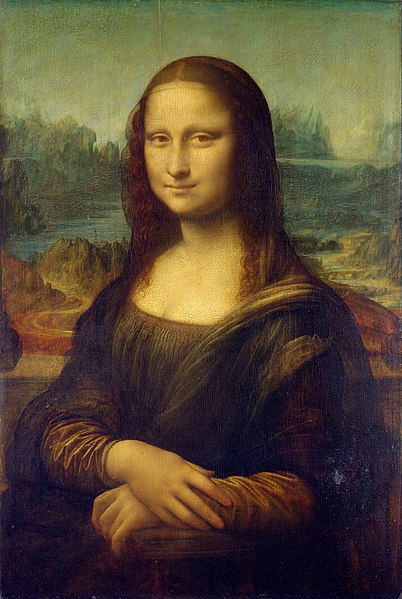
\includegraphics[width=0.4\textwidth]{monalisa}
	\caption[Mona Lisa, again]{It's Mona Lisa again. \blindtext}
	\labfig{normalmonalisa}
\end{figure}

The tables can be inserted as easily as the figures, as exemplified in 
the following code:

\begin{lstlisting}
\begin{table}
\begin{tabular}{ c c c c  }
	\toprule
	col1 & col2 & col3 \\
	\midrule
	\multirow{3}{4em}{Multiple row} & cell2 & cell3 \\ &
	cell5 & cell6 \\ &
	cell8 & cell9 \\
	\bottomrule
\end{tabular}
\caption[A useless table]{A useless table.}
\end{table}
\end{lstlisting}

which results in the useless \reftab{useless}.

\begin{table}[h]
\begin{tabular}{ c c c c  }
	\toprule
	col1 & col2 & col3 \\
	\midrule
	\multirow{3}{4em}{Multiple row} & cell2 & cell3 \\ &
	cell5 & cell6 \\ &
	cell8 & cell9 \\
	\bottomrule
\end{tabular}
\caption[A useless table]{A useless table.}
\labtab{useless}
\end{table}

I don't have much else to say, so I will just insert some blind text. 
\blindtext

\section{Margin figures and tables}

Marginfigures can be inserted with the environment \verb|marginfigure|. 
In this case, the whole picture is confined to the margin and the 
caption is below it. \reffig{marginmonalisa} is obtained with something 
like this:

\begin{lstlisting}
\begin{marginfigure}
	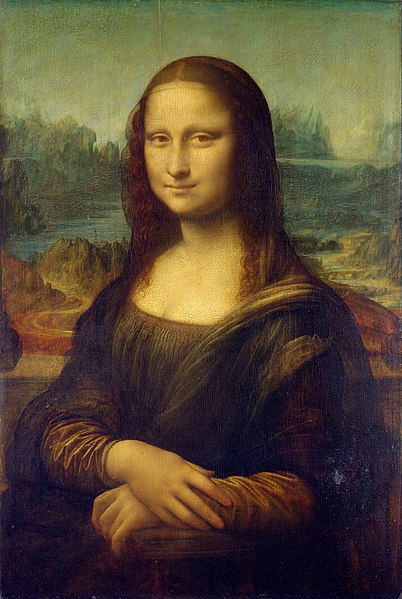
\includegraphics{monalisa}
	\caption[The Mona Lisa]{The Mona Lisa.}
	\labfig{marginmonalisa}
\end{marginfigure}
\end{lstlisting}

There is also the \verb|margintable| environment, of which 
\reftab{anotheruseless} is an example.

\begin{margintable}
\raggedright
\begin{tabular}{ c c c c }
	\hline
	col1 & col2 & col3 \\
	\hline
	\multirow{3}{4em}{Multiple row} & cell2 & cell3 \\ & cell5 & cell6 
	\\ & cell8 & cell9 \\ \hline
\end{tabular}
\caption[Another useless table]{Another useless table.}
\labtab{anotheruseless}
\end{margintable}

Marginfigures and tables can be positioned with an optional offset 
command, like so:

\begin{lstlisting}
\begin{marginfigure}[offset]
	\includegraphics{images/seaside}
\end{marginfigure}
\end{lstlisting}

Offset ca be either a measure or a multiple of \verb|\baselineskip|, 
much like with \verb|\sidenote|, \verb|\marginnote| and 
\verb|\margintoc|.\todo{improve this part} If you are wondering how I 
inserted this orange bubble, have a look at the \verb|todo| package.

\section{Wide figures and tables}

With the environments \verb|figure*| and \verb|table*| you can insert 
figures which span the whole page width. The caption will be positioned 
below.

\begin{figure*}[h!]
	\includegraphics{seaside}
	\vspace*{-1.3cm}
	\caption[A wide seaside]{A wide seaside, and a wide caption.
		Credits: By Bushra Feroz - Own work, CC BY-SA 4.0, 
		https://commons.wikimedia.org/w/index.php?curid=68724647.
		\blindtext}
\end{figure*}

\section{Image before chapter}

It is relatively easy to insert a figure before the chapter title with 
the help of the \verb|\setchapterpreamble| command. The details are left 
to the reader.\sidenote{Check the source code for a hint.}

In this chapter I also have used a different chapter title style. This 
is just to demonstrate how easy it is to alter the default if you don't 
like it and if you are willing to write some commands on your own. For 
instance, you could try the following code:

\begin{lstlisting}
\renewcommand*{\chapterformat}
{
  \enskip\mbox{\scalebox{3.5}{\framebox{\thechapter\autodot}}}
}
\renewcommand\chapterlinesformat[3]
{
  \parbox[b]{\textwidth+\marginparsep+\marginparwidth}{
	\parbox[b]{\textwidth}{#3}%
	\parbox[b]{\marginparsep}{\hfill}%
	\parbox[b]{\marginparwidth}{#2}%
  }
  %\hrule
}
\end{lstlisting}
